\documentclass{standalone}
\usepackage{tikz}
\usetikzlibrary{patterns}
\usetikzlibrary{positioning}
\usetikzlibrary{patterns, positioning}
\usetikzlibrary{shapes.misc}
\usepackage[outline]{contour}
\contourlength{1.5pt} 
\usetikzlibrary{calc}
        \usepackage{relsize}
        \tikzset{fontscale/.style = {font=\relsize{#1}}}

\begin{document}
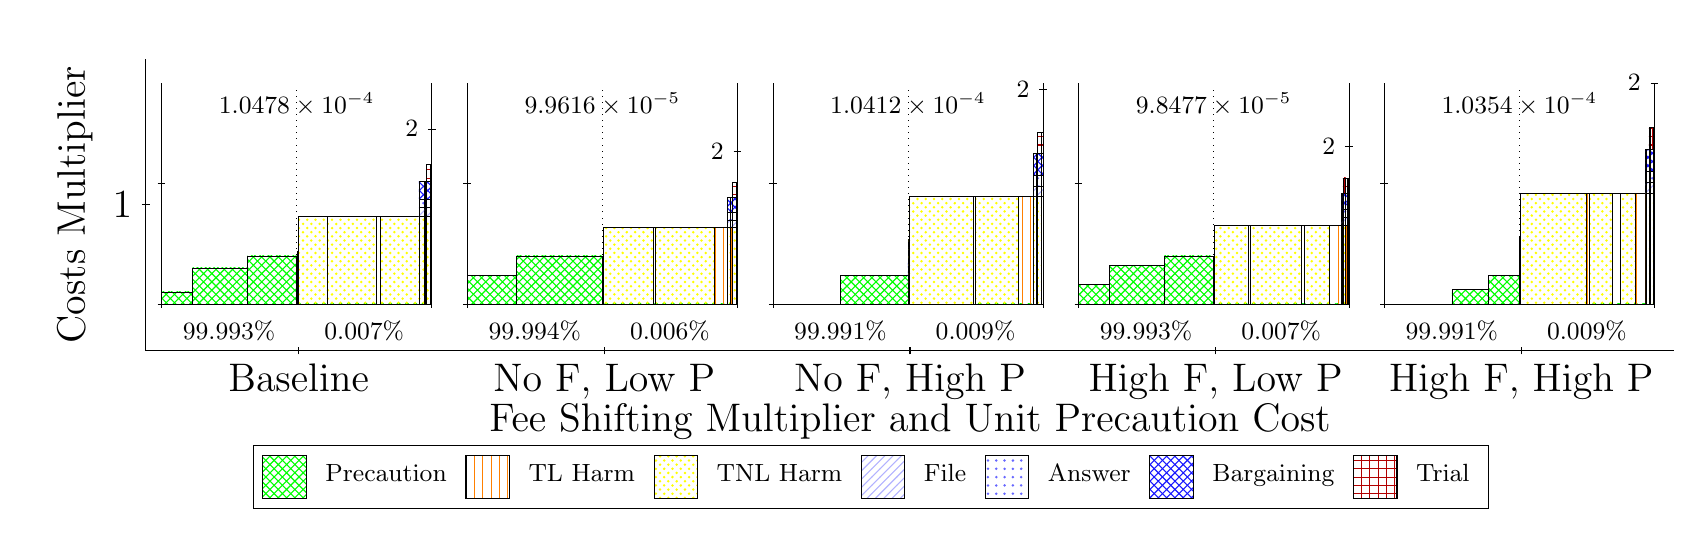
\begin{tikzpicture}
\clip(-0.5,-1.1) rectangle +(20.91,6.2);
\draw[black] (1,1) -- (1,4.7);
\node[rotate=90, fontscale=2, anchor=center] at (0.1, 2.85) {Costs Multiplier};
\draw[black] (0.95,2.85) -- (1.05,2.85);
\node[fontscale=2, anchor=east] at (0.95, 2.85) {1};

\draw[black] (1,1) -- (20.41,1);
\node[fontscale=2, anchor=center] at (10.705, 0.1) {Fee Shifting Multiplier and Unit Precaution Cost};
\draw[black] (2.941,0.95) -- (2.941,1.05);
\node[fontscale=2, anchor=north] at (2.941, 0.95) {Baseline};
\draw[black] (6.823,0.95) -- (6.823,1.05);
\node[fontscale=2, anchor=north] at (6.823, 0.95) {No F, Low P};
\draw[black] (10.705,0.95) -- (10.705,1.05);
\node[fontscale=2, anchor=north] at (10.705, 0.95) {No F, High P};
\draw[black] (14.587,0.95) -- (14.587,1.05);
\node[fontscale=2, anchor=north] at (14.587, 0.95) {High F, Low P};
\draw[black] (18.469,0.95) -- (18.469,1.05);
\node[fontscale=2, anchor=north] at (18.469, 0.95) {High F, High P};


\draw[pattern=crosshatch, pattern color=green,draw=black,very thin] (1.2,1.592) rectangle (1.5947,1.7447);
\draw[pattern=crosshatch, pattern color=green,draw=black,very thin] (1.5947,1.592) rectangle (2.2894,2.0501);
\draw[pattern=crosshatch, pattern color=green,draw=black,very thin] (2.2894,1.592) rectangle (2.916,2.2028);
\draw[pattern=crosshatch, pattern color=green,draw=black,very thin] (2.916,1.592) rectangle (2.9243,1.592);
\draw[pattern=north east lines, pattern color=blue!30,draw=black,very thin] (2.916,1.592) rectangle (2.9243,1.7032);
\draw[pattern=dots,  pattern color=blue!60,draw=black,very thin] (2.916,1.7032) rectangle (2.9243,1.8143);
\draw[pattern=crosshatch,      pattern color=blue!90,draw=black,very thin] (2.916,1.8143) rectangle (2.9243,2.0366);
\draw[pattern=crosshatch, pattern color=green,draw=black,very thin] (2.9243,1.592) rectangle (2.9274,1.592);
\draw[pattern=north east lines, pattern color=blue!30,draw=black,very thin] (2.9243,1.592) rectangle (2.9274,1.7032);
\draw[pattern=dots,  pattern color=blue!60,draw=black,very thin] (2.9243,1.7032) rectangle (2.9274,1.8143);
\draw[pattern=crosshatch,      pattern color=blue!90,draw=black,very thin] (2.9243,1.8143) rectangle (2.9274,2.0367);
\draw[pattern=crosshatch, pattern color=green,draw=black,very thin] (2.9274,1.592) rectangle (2.9334,1.592);
\draw[pattern=north east lines, pattern color=blue!30,draw=black,very thin] (2.9274,1.592) rectangle (2.9334,1.7032);
\draw[pattern=dots,  pattern color=blue!60,draw=black,very thin] (2.9274,1.7032) rectangle (2.9334,1.8143);
\draw[pattern=crosshatch,      pattern color=blue!90,draw=black,very thin] (2.9274,1.8143) rectangle (2.9334,2.0366);
\draw[pattern=grid,            pattern color=red!70!black,draw=black,very thin] (2.9274,2.0366) rectangle (2.9334,2.2589);
\draw[pattern=crosshatch, pattern color=green,draw=black,very thin] (2.9334,1.592) rectangle (2.9354,1.592);
\draw[pattern=north east lines, pattern color=blue!30,draw=black,very thin] (2.9334,1.592) rectangle (2.9354,1.7032);
\draw[pattern=dots,  pattern color=blue!60,draw=black,very thin] (2.9334,1.7032) rectangle (2.9354,1.8143);
\draw[pattern=crosshatch,      pattern color=blue!90,draw=black,very thin] (2.9334,1.8143) rectangle (2.9354,2.0367);
\draw[pattern=grid,            pattern color=red!70!black,draw=black,very thin] (2.9334,2.0367) rectangle (2.9354,2.259);
\draw[pattern=crosshatch, pattern color=green,draw=black,very thin] (2.9354,1.592) rectangle (3.3039,1.592);
\draw[pattern=crosshatch dots, pattern color=yellow,draw=black,very thin] (2.9354,1.592) rectangle (3.3039,2.7036);
\draw[pattern=crosshatch, pattern color=green,draw=black,very thin] (3.3039,1.592) rectangle (3.3061,1.592);
\draw[pattern=vertical lines, pattern color=orange,draw=black,very thin] (3.3039,1.592) rectangle (3.3061,2.7036);
\draw[pattern=crosshatch, pattern color=green,draw=black,very thin] (3.3061,1.592) rectangle (3.9318,1.592);
\draw[pattern=crosshatch dots, pattern color=yellow,draw=black,very thin] (3.3061,1.592) rectangle (3.9318,2.7036);
\draw[pattern=crosshatch, pattern color=green,draw=black,very thin] (3.9318,1.592) rectangle (3.977,1.592);
\draw[pattern=vertical lines, pattern color=orange,draw=black,very thin] (3.9318,1.592) rectangle (3.977,2.7036);
\draw[pattern=crosshatch, pattern color=green,draw=black,very thin] (3.977,1.592) rectangle (4.4677,1.592);
\draw[pattern=crosshatch dots, pattern color=yellow,draw=black,very thin] (3.977,1.592) rectangle (4.4677,2.7036);
\draw[pattern=crosshatch, pattern color=green,draw=black,very thin] (4.4677,1.592) rectangle (4.5339,1.592);
\draw[pattern=crosshatch dots, pattern color=yellow,draw=black,very thin] (4.4677,1.592) rectangle (4.5339,2.7036);
\draw[pattern=north east lines, pattern color=blue!30,draw=black,very thin] (4.4677,2.7036) rectangle (4.5339,2.8147);
\draw[pattern=dots,  pattern color=blue!60,draw=black,very thin] (4.4677,2.8147) rectangle (4.5339,2.9259);
\draw[pattern=crosshatch,      pattern color=blue!90,draw=black,very thin] (4.4677,2.9259) rectangle (4.5339,3.1482);
\draw[pattern=crosshatch, pattern color=green,draw=black,very thin] (4.5339,1.592) rectangle (4.5435,1.592);
\draw[pattern=vertical lines, pattern color=orange,draw=black,very thin] (4.5339,1.592) rectangle (4.5435,2.7036);
\draw[pattern=north east lines, pattern color=blue!30,draw=black,very thin] (4.5339,2.7036) rectangle (4.5435,2.8147);
\draw[pattern=dots,  pattern color=blue!60,draw=black,very thin] (4.5339,2.8147) rectangle (4.5435,2.9259);
\draw[pattern=crosshatch,      pattern color=blue!90,draw=black,very thin] (4.5339,2.9259) rectangle (4.5435,3.1482);
\draw[pattern=crosshatch, pattern color=green,draw=black,very thin] (4.5435,1.592) rectangle (4.5503,1.592);
\draw[pattern=crosshatch dots, pattern color=yellow,draw=black,very thin] (4.5435,1.592) rectangle (4.5503,2.7036);
\draw[pattern=north east lines, pattern color=blue!30,draw=black,very thin] (4.5435,2.7036) rectangle (4.5503,2.8147);
\draw[pattern=dots,  pattern color=blue!60,draw=black,very thin] (4.5435,2.8147) rectangle (4.5503,2.9259);
\draw[pattern=crosshatch,      pattern color=blue!90,draw=black,very thin] (4.5435,2.9259) rectangle (4.5503,3.1482);
\draw[pattern=crosshatch, pattern color=green,draw=black,very thin] (4.5503,1.592) rectangle (4.5634,1.592);
\draw[pattern=vertical lines, pattern color=orange,draw=black,very thin] (4.5503,1.592) rectangle (4.5634,2.7036);
\draw[pattern=north east lines, pattern color=blue!30,draw=black,very thin] (4.5503,2.7036) rectangle (4.5634,2.8147);
\draw[pattern=dots,  pattern color=blue!60,draw=black,very thin] (4.5503,2.8147) rectangle (4.5634,2.9259);
\draw[pattern=crosshatch,      pattern color=blue!90,draw=black,very thin] (4.5503,2.9259) rectangle (4.5634,3.1482);
\draw[pattern=crosshatch, pattern color=green,draw=black,very thin] (4.5634,1.592) rectangle (4.612,1.592);
\draw[pattern=crosshatch dots, pattern color=yellow,draw=black,very thin] (4.5634,1.592) rectangle (4.612,2.7036);
\draw[pattern=north east lines, pattern color=blue!30,draw=black,very thin] (4.5634,2.7036) rectangle (4.612,2.8147);
\draw[pattern=dots,  pattern color=blue!60,draw=black,very thin] (4.5634,2.8147) rectangle (4.612,2.9259);
\draw[pattern=crosshatch,      pattern color=blue!90,draw=black,very thin] (4.5634,2.9259) rectangle (4.612,3.1482);
\draw[pattern=grid,            pattern color=red!70!black,draw=black,very thin] (4.5634,3.1482) rectangle (4.612,3.3705);
\draw[pattern=crosshatch, pattern color=green,draw=black,very thin] (4.612,1.592) rectangle (4.6185,1.592);
\draw[pattern=vertical lines, pattern color=orange,draw=black,very thin] (4.612,1.592) rectangle (4.6185,2.7036);
\draw[pattern=north east lines, pattern color=blue!30,draw=black,very thin] (4.612,2.7036) rectangle (4.6185,2.8147);
\draw[pattern=dots,  pattern color=blue!60,draw=black,very thin] (4.612,2.8147) rectangle (4.6185,2.9259);
\draw[pattern=crosshatch,      pattern color=blue!90,draw=black,very thin] (4.612,2.9259) rectangle (4.6185,3.1482);
\draw[pattern=grid,            pattern color=red!70!black,draw=black,very thin] (4.612,3.1482) rectangle (4.6185,3.3705);
\draw[pattern=crosshatch, pattern color=green,draw=black,very thin] (4.6185,1.592) rectangle (4.6264,1.592);
\draw[pattern=crosshatch dots, pattern color=yellow,draw=black,very thin] (4.6185,1.592) rectangle (4.6264,2.7036);
\draw[pattern=north east lines, pattern color=blue!30,draw=black,very thin] (4.6185,2.7036) rectangle (4.6264,2.8147);
\draw[pattern=dots,  pattern color=blue!60,draw=black,very thin] (4.6185,2.8147) rectangle (4.6264,2.9259);
\draw[pattern=crosshatch,      pattern color=blue!90,draw=black,very thin] (4.6185,2.9259) rectangle (4.6264,3.1482);
\draw[pattern=grid,            pattern color=red!70!black,draw=black,very thin] (4.6185,3.1482) rectangle (4.6264,3.3705);
\draw[pattern=crosshatch, pattern color=green,draw=black,very thin] (4.6264,1.592) rectangle (4.632,1.592);
\draw[pattern=vertical lines, pattern color=orange,draw=black,very thin] (4.6264,1.592) rectangle (4.632,2.7036);
\draw[pattern=north east lines, pattern color=blue!30,draw=black,very thin] (4.6264,2.7036) rectangle (4.632,2.8147);
\draw[pattern=dots,  pattern color=blue!60,draw=black,very thin] (4.6264,2.8147) rectangle (4.632,2.9259);
\draw[pattern=crosshatch,      pattern color=blue!90,draw=black,very thin] (4.6264,2.9259) rectangle (4.632,3.1482);
\draw[pattern=grid,            pattern color=red!70!black,draw=black,very thin] (4.6264,3.1482) rectangle (4.632,3.3705);
\node[font=\small,text=black,anchor=north] at (2.916, 4.4) {$1.0478\times 10^{-4}$};
\draw[black,very thin] (1.2,1.592) -- (1.2,4.4);
\draw[black,very thin] (1.15,1.592) -- (1.25,1.592);
\node[font=\small,text=black, anchor=west] at (1.15, 1.592) {};
\draw[black,very thin] (1.15,3.1191) -- (1.25,3.1191);
\node[font=\small,text=black, anchor=west] at (1.15, 3.1191) {};

\draw[black,dotted,very thin] (2.916,1.6762) -- (2.916,4.3158);
\draw[black,very thin] (4.632,1.592) -- (4.632,4.4);
\draw[black,very thin] (4.582,3.8151) -- (4.682,3.8151);
\node[font=\small,text=black, anchor=east] at (4.582, 3.8151) {\contour{white}{2}};

\draw[black,very thin] (1.2,1.592) -- (4.632,1.592);
\draw[black,very thin] (1.2,1.542) -- (1.2,1.642);
\node[font=\small,text=black, anchor=north] at (1.2, 1.542) {};
\draw[black,very thin] (4.632,1.542) -- (4.632,1.642);
\node[font=\small,text=black, anchor=north] at (4.632, 1.542) {};

\node[font=\small,text=black,anchor=south] at (2.058, 0.992) {99.993\%};
\node[font=\small,text=black,anchor=south] at (3.774, 0.992) {0.007\%};

\draw[pattern=crosshatch, pattern color=green,draw=black,very thin] (5.082,1.592) rectangle (5.7085,1.9585);
\draw[pattern=crosshatch, pattern color=green,draw=black,very thin] (5.7085,1.592) rectangle (6.798,2.2028);
\draw[pattern=crosshatch, pattern color=green,draw=black,very thin] (6.798,1.592) rectangle (6.8067,1.592);
\draw[pattern=north east lines, pattern color=blue!30,draw=black,very thin] (6.798,1.592) rectangle (6.8067,1.6889);
\draw[pattern=dots,  pattern color=blue!60,draw=black,very thin] (6.798,1.6889) rectangle (6.8067,1.7858);
\draw[pattern=crosshatch,      pattern color=blue!90,draw=black,very thin] (6.798,1.7858) rectangle (6.8067,1.9795);
\draw[pattern=crosshatch, pattern color=green,draw=black,very thin] (6.8067,1.592) rectangle (6.8152,1.592);
\draw[pattern=north east lines, pattern color=blue!30,draw=black,very thin] (6.8067,1.592) rectangle (6.8152,1.6889);
\draw[pattern=dots,  pattern color=blue!60,draw=black,very thin] (6.8067,1.6889) rectangle (6.8152,1.7858);
\draw[pattern=crosshatch,      pattern color=blue!90,draw=black,very thin] (6.8067,1.7858) rectangle (6.8152,1.9795);
\draw[pattern=grid,            pattern color=red!70!black,draw=black,very thin] (6.8067,1.9795) rectangle (6.8152,2.1733);
\draw[pattern=crosshatch, pattern color=green,draw=black,very thin] (6.8152,1.592) rectangle (7.4506,1.592);
\draw[pattern=crosshatch dots, pattern color=yellow,draw=black,very thin] (6.8152,1.592) rectangle (7.4506,2.5608);
\draw[pattern=crosshatch, pattern color=green,draw=black,very thin] (7.4506,1.592) rectangle (7.4681,1.592);
\draw[pattern=vertical lines, pattern color=orange,draw=black,very thin] (7.4506,1.592) rectangle (7.4681,2.5608);
\draw[pattern=crosshatch, pattern color=green,draw=black,very thin] (7.4681,1.592) rectangle (8.2135,1.592);
\draw[pattern=crosshatch dots, pattern color=yellow,draw=black,very thin] (7.4681,1.592) rectangle (8.2135,2.5608);
\draw[pattern=crosshatch, pattern color=green,draw=black,very thin] (8.2135,1.592) rectangle (8.3872,1.592);
\draw[pattern=vertical lines, pattern color=orange,draw=black,very thin] (8.2135,1.592) rectangle (8.3872,2.5608);
\draw[pattern=crosshatch, pattern color=green,draw=black,very thin] (8.3872,1.592) rectangle (8.4233,1.592);
\draw[pattern=crosshatch dots, pattern color=yellow,draw=black,very thin] (8.3872,1.592) rectangle (8.4233,2.5608);
\draw[pattern=north east lines, pattern color=blue!30,draw=black,very thin] (8.3872,2.5608) rectangle (8.4233,2.6576);
\draw[pattern=dots,  pattern color=blue!60,draw=black,very thin] (8.3872,2.6576) rectangle (8.4233,2.7545);
\draw[pattern=crosshatch,      pattern color=blue!90,draw=black,very thin] (8.3872,2.7545) rectangle (8.4233,2.9483);
\draw[pattern=crosshatch, pattern color=green,draw=black,very thin] (8.4233,1.592) rectangle (8.4506,1.592);
\draw[pattern=vertical lines, pattern color=orange,draw=black,very thin] (8.4233,1.592) rectangle (8.4506,2.5608);
\draw[pattern=north east lines, pattern color=blue!30,draw=black,very thin] (8.4233,2.5608) rectangle (8.4506,2.6576);
\draw[pattern=dots,  pattern color=blue!60,draw=black,very thin] (8.4233,2.6576) rectangle (8.4506,2.7545);
\draw[pattern=crosshatch,      pattern color=blue!90,draw=black,very thin] (8.4233,2.7545) rectangle (8.4506,2.9483);
\draw[pattern=crosshatch, pattern color=green,draw=black,very thin] (8.4506,1.592) rectangle (8.498,1.592);
\draw[pattern=crosshatch dots, pattern color=yellow,draw=black,very thin] (8.4506,1.592) rectangle (8.498,2.5608);
\draw[pattern=north east lines, pattern color=blue!30,draw=black,very thin] (8.4506,2.5608) rectangle (8.498,2.6576);
\draw[pattern=dots,  pattern color=blue!60,draw=black,very thin] (8.4506,2.6576) rectangle (8.498,2.7545);
\draw[pattern=crosshatch,      pattern color=blue!90,draw=black,very thin] (8.4506,2.7545) rectangle (8.498,2.9483);
\draw[pattern=grid,            pattern color=red!70!black,draw=black,very thin] (8.4506,2.9483) rectangle (8.498,3.142);
\draw[pattern=crosshatch, pattern color=green,draw=black,very thin] (8.498,1.592) rectangle (8.514,1.592);
\draw[pattern=vertical lines, pattern color=orange,draw=black,very thin] (8.498,1.592) rectangle (8.514,2.5608);
\draw[pattern=north east lines, pattern color=blue!30,draw=black,very thin] (8.498,2.5608) rectangle (8.514,2.6576);
\draw[pattern=dots,  pattern color=blue!60,draw=black,very thin] (8.498,2.6576) rectangle (8.514,2.7545);
\draw[pattern=crosshatch,      pattern color=blue!90,draw=black,very thin] (8.498,2.7545) rectangle (8.514,2.9483);
\draw[pattern=grid,            pattern color=red!70!black,draw=black,very thin] (8.498,2.9483) rectangle (8.514,3.142);
\node[font=\small,text=black,anchor=north] at (6.798, 4.4) {$9.9616\times 10^{-5}$};
\draw[black,very thin] (5.082,1.592) -- (5.082,4.4);
\draw[black,very thin] (5.032,1.592) -- (5.132,1.592);
\node[font=\small,text=black, anchor=west] at (5.032, 1.592) {};
\draw[black,very thin] (5.032,3.1191) -- (5.132,3.1191);
\node[font=\small,text=black, anchor=west] at (5.032, 3.1191) {};

\draw[black,dotted,very thin] (6.798,1.6762) -- (6.798,4.3158);
\draw[black,very thin] (8.514,1.592) -- (8.514,4.4);
\draw[black,very thin] (8.464,3.5295) -- (8.564,3.5295);
\node[font=\small,text=black, anchor=east] at (8.464, 3.5295) {\contour{white}{2}};

\draw[black,very thin] (5.082,1.592) -- (8.514,1.592);
\draw[black,very thin] (5.082,1.542) -- (5.082,1.642);
\node[font=\small,text=black, anchor=north] at (5.082, 1.542) {};
\draw[black,very thin] (8.514,1.542) -- (8.514,1.642);
\node[font=\small,text=black, anchor=north] at (8.514, 1.542) {};

\node[font=\small,text=black,anchor=south] at (5.94, 0.992) {99.994\%};
\node[font=\small,text=black,anchor=south] at (7.656, 0.992) {0.006\%};

\draw[pattern=crosshatch, pattern color=green,draw=black,very thin] (9.822,1.592) rectangle (10.68,1.9585);
\draw[pattern=north east lines, pattern color=blue!30,draw=black,very thin] (10.68,1.592) rectangle (10.685,1.7282);
\draw[pattern=dots,  pattern color=blue!60,draw=black,very thin] (10.68,1.7282) rectangle (10.685,1.8644);
\draw[pattern=crosshatch,      pattern color=blue!90,draw=black,very thin] (10.68,1.8644) rectangle (10.685,2.1367);
\draw[pattern=north east lines, pattern color=blue!30,draw=black,very thin] (10.685,1.592) rectangle (10.692,1.7282);
\draw[pattern=dots,  pattern color=blue!60,draw=black,very thin] (10.685,1.7282) rectangle (10.692,1.8644);
\draw[pattern=crosshatch,      pattern color=blue!90,draw=black,very thin] (10.685,1.8644) rectangle (10.692,2.1367);
\draw[pattern=grid,            pattern color=red!70!black,draw=black,very thin] (10.685,2.1367) rectangle (10.692,2.4091);
\draw[pattern=crosshatch dots, pattern color=yellow,draw=black,very thin] (10.692,1.592) rectangle (11.512,2.9538);
\draw[pattern=vertical lines, pattern color=orange,draw=black,very thin] (11.512,1.592) rectangle (11.532,2.9538);
\draw[pattern=crosshatch, pattern color=green,draw=black,very thin] (11.532,1.592) rectangle (12.08,1.592);
\draw[pattern=crosshatch dots, pattern color=yellow,draw=black,very thin] (11.532,1.592) rectangle (12.08,2.9538);
\draw[pattern=crosshatch, pattern color=green,draw=black,very thin] (12.08,1.592) rectangle (12.274,1.592);
\draw[pattern=vertical lines, pattern color=orange,draw=black,very thin] (12.08,1.592) rectangle (12.274,2.9538);
\draw[pattern=crosshatch dots, pattern color=yellow,draw=black,very thin] (12.274,1.592) rectangle (12.303,2.9538);
\draw[pattern=north east lines, pattern color=blue!30,draw=black,very thin] (12.274,2.9538) rectangle (12.303,3.0899);
\draw[pattern=dots,  pattern color=blue!60,draw=black,very thin] (12.274,3.0899) rectangle (12.303,3.2261);
\draw[pattern=crosshatch,      pattern color=blue!90,draw=black,very thin] (12.274,3.2261) rectangle (12.303,3.4985);
\draw[pattern=vertical lines, pattern color=orange,draw=black,very thin] (12.303,1.592) rectangle (12.327,2.9538);
\draw[pattern=north east lines, pattern color=blue!30,draw=black,very thin] (12.303,2.9538) rectangle (12.327,3.0899);
\draw[pattern=dots,  pattern color=blue!60,draw=black,very thin] (12.303,3.0899) rectangle (12.327,3.2261);
\draw[pattern=crosshatch,      pattern color=blue!90,draw=black,very thin] (12.303,3.2261) rectangle (12.327,3.4985);
\draw[pattern=crosshatch dots, pattern color=yellow,draw=black,very thin] (12.327,1.592) rectangle (12.374,2.9538);
\draw[pattern=north east lines, pattern color=blue!30,draw=black,very thin] (12.327,2.9538) rectangle (12.374,3.0899);
\draw[pattern=dots,  pattern color=blue!60,draw=black,very thin] (12.327,3.0899) rectangle (12.374,3.2261);
\draw[pattern=crosshatch,      pattern color=blue!90,draw=black,very thin] (12.327,3.2261) rectangle (12.374,3.4985);
\draw[pattern=grid,            pattern color=red!70!black,draw=black,very thin] (12.327,3.4985) rectangle (12.374,3.7708);
\draw[pattern=vertical lines, pattern color=orange,draw=black,very thin] (12.374,1.592) rectangle (12.396,2.9538);
\draw[pattern=north east lines, pattern color=blue!30,draw=black,very thin] (12.374,2.9538) rectangle (12.396,3.0899);
\draw[pattern=dots,  pattern color=blue!60,draw=black,very thin] (12.374,3.0899) rectangle (12.396,3.2261);
\draw[pattern=crosshatch,      pattern color=blue!90,draw=black,very thin] (12.374,3.2261) rectangle (12.396,3.4985);
\draw[pattern=grid,            pattern color=red!70!black,draw=black,very thin] (12.374,3.4985) rectangle (12.396,3.7708);
\node[font=\small,text=black,anchor=north] at (10.68, 4.4) {$1.0412\times 10^{-4}$};
\draw[black,very thin] (8.964,1.592) -- (8.964,4.4);
\draw[black,very thin] (8.914,1.592) -- (9.014,1.592);
\node[font=\small,text=black, anchor=west] at (8.914, 1.592) {};
\draw[black,very thin] (8.914,3.1191) -- (9.014,3.1191);
\node[font=\small,text=black, anchor=west] at (8.914, 3.1191) {};

\draw[black,dotted,very thin] (10.68,1.6762) -- (10.68,4.3158);
\draw[black,very thin] (12.396,1.592) -- (12.396,4.4);
\draw[black,very thin] (12.346,4.3155) -- (12.446,4.3155);
\node[font=\small,text=black, anchor=east] at (12.346, 4.3155) {\contour{white}{2}};

\draw[black,very thin] (8.964,1.592) -- (12.396,1.592);
\draw[black,very thin] (8.964,1.542) -- (8.964,1.642);
\node[font=\small,text=black, anchor=north] at (8.964, 1.542) {};
\draw[black,very thin] (12.396,1.542) -- (12.396,1.642);
\node[font=\small,text=black, anchor=north] at (12.396, 1.542) {};

\node[font=\small,text=black,anchor=south] at (9.822, 0.992) {99.991\%};
\node[font=\small,text=black,anchor=south] at (11.538, 0.992) {0.009\%};

\draw[pattern=crosshatch, pattern color=green,draw=black,very thin] (12.846,1.592) rectangle (13.241,1.8363);
\draw[pattern=crosshatch, pattern color=green,draw=black,very thin] (13.241,1.592) rectangle (13.935,2.0807);
\draw[pattern=crosshatch, pattern color=green,draw=black,very thin] (13.935,1.592) rectangle (14.562,2.2028);
\draw[pattern=crosshatch, pattern color=green,draw=black,very thin] (14.562,1.592) rectangle (14.565,1.592);
\draw[pattern=north east lines, pattern color=blue!30,draw=black,very thin] (14.562,1.592) rectangle (14.565,1.692);
\draw[pattern=dots,  pattern color=blue!60,draw=black,very thin] (14.562,1.692) rectangle (14.565,1.7919);
\draw[pattern=crosshatch,      pattern color=blue!90,draw=black,very thin] (14.562,1.7919) rectangle (14.565,1.9918);
\draw[pattern=crosshatch, pattern color=green,draw=black,very thin] (14.565,1.592) rectangle (14.573,1.592);
\draw[pattern=north east lines, pattern color=blue!30,draw=black,very thin] (14.565,1.592) rectangle (14.573,1.692);
\draw[pattern=dots,  pattern color=blue!60,draw=black,very thin] (14.565,1.692) rectangle (14.573,1.7919);
\draw[pattern=crosshatch,      pattern color=blue!90,draw=black,very thin] (14.565,1.7919) rectangle (14.573,1.9918);
\draw[pattern=grid,            pattern color=red!70!black,draw=black,very thin] (14.565,1.9918) rectangle (14.573,2.1917);
\draw[pattern=crosshatch, pattern color=green,draw=black,very thin] (14.573,1.592) rectangle (14.575,1.592);
\draw[pattern=north east lines, pattern color=blue!30,draw=black,very thin] (14.573,1.592) rectangle (14.575,1.692);
\draw[pattern=dots,  pattern color=blue!60,draw=black,very thin] (14.573,1.692) rectangle (14.575,1.7919);
\draw[pattern=crosshatch,      pattern color=blue!90,draw=black,very thin] (14.573,1.7919) rectangle (14.575,1.9918);
\draw[pattern=grid,            pattern color=red!70!black,draw=black,very thin] (14.573,1.9918) rectangle (14.575,2.1917);
\draw[pattern=crosshatch, pattern color=green,draw=black,very thin] (14.575,1.592) rectangle (15,1.592);
\draw[pattern=crosshatch dots, pattern color=yellow,draw=black,very thin] (14.575,1.592) rectangle (15,2.5914);
\draw[pattern=crosshatch, pattern color=green,draw=black,very thin] (15,1.592) rectangle (15.03,1.592);
\draw[pattern=vertical lines, pattern color=orange,draw=black,very thin] (15,1.592) rectangle (15.03,2.5914);
\draw[pattern=crosshatch, pattern color=green,draw=black,very thin] (15.03,1.592) rectangle (15.669,1.592);
\draw[pattern=crosshatch dots, pattern color=yellow,draw=black,very thin] (15.03,1.592) rectangle (15.669,2.5915);
\draw[pattern=crosshatch, pattern color=green,draw=black,very thin] (15.669,1.592) rectangle (15.711,1.592);
\draw[pattern=vertical lines, pattern color=orange,draw=black,very thin] (15.669,1.592) rectangle (15.711,2.5915);
\draw[pattern=crosshatch, pattern color=green,draw=black,very thin] (15.711,1.592) rectangle (16.031,1.592);
\draw[pattern=crosshatch dots, pattern color=yellow,draw=black,very thin] (15.711,1.592) rectangle (16.031,2.5915);
\draw[pattern=crosshatch, pattern color=green,draw=black,very thin] (16.031,1.592) rectangle (16.183,1.592);
\draw[pattern=vertical lines, pattern color=orange,draw=black,very thin] (16.031,1.592) rectangle (16.183,2.5915);
\draw[pattern=crosshatch, pattern color=green,draw=black,very thin] (16.183,1.592) rectangle (16.19,1.592);
\draw[pattern=crosshatch dots, pattern color=yellow,draw=black,very thin] (16.183,1.592) rectangle (16.19,2.5915);
\draw[pattern=north east lines, pattern color=blue!30,draw=black,very thin] (16.183,2.5915) rectangle (16.19,2.6914);
\draw[pattern=dots,  pattern color=blue!60,draw=black,very thin] (16.183,2.6914) rectangle (16.19,2.7914);
\draw[pattern=crosshatch,      pattern color=blue!90,draw=black,very thin] (16.183,2.7914) rectangle (16.19,2.9912);
\draw[pattern=crosshatch, pattern color=green,draw=black,very thin] (16.19,1.592) rectangle (16.202,1.592);
\draw[pattern=vertical lines, pattern color=orange,draw=black,very thin] (16.19,1.592) rectangle (16.202,2.5915);
\draw[pattern=north east lines, pattern color=blue!30,draw=black,very thin] (16.19,2.5915) rectangle (16.202,2.6914);
\draw[pattern=dots,  pattern color=blue!60,draw=black,very thin] (16.19,2.6914) rectangle (16.202,2.7914);
\draw[pattern=crosshatch,      pattern color=blue!90,draw=black,very thin] (16.19,2.7914) rectangle (16.202,2.9912);
\draw[pattern=crosshatch, pattern color=green,draw=black,very thin] (16.202,1.592) rectangle (16.235,1.592);
\draw[pattern=crosshatch dots, pattern color=yellow,draw=black,very thin] (16.202,1.592) rectangle (16.235,2.5914);
\draw[pattern=north east lines, pattern color=blue!30,draw=black,very thin] (16.202,2.5914) rectangle (16.235,2.6914);
\draw[pattern=dots,  pattern color=blue!60,draw=black,very thin] (16.202,2.6914) rectangle (16.235,2.7913);
\draw[pattern=crosshatch,      pattern color=blue!90,draw=black,very thin] (16.202,2.7913) rectangle (16.235,2.9912);
\draw[pattern=grid,            pattern color=red!70!black,draw=black,very thin] (16.202,2.9912) rectangle (16.235,3.1911);
\draw[pattern=crosshatch, pattern color=green,draw=black,very thin] (16.235,1.592) rectangle (16.265,1.592);
\draw[pattern=vertical lines, pattern color=orange,draw=black,very thin] (16.235,1.592) rectangle (16.265,2.5914);
\draw[pattern=north east lines, pattern color=blue!30,draw=black,very thin] (16.235,2.5914) rectangle (16.265,2.6914);
\draw[pattern=dots,  pattern color=blue!60,draw=black,very thin] (16.235,2.6914) rectangle (16.265,2.7913);
\draw[pattern=crosshatch,      pattern color=blue!90,draw=black,very thin] (16.235,2.7913) rectangle (16.265,2.9912);
\draw[pattern=grid,            pattern color=red!70!black,draw=black,very thin] (16.235,2.9912) rectangle (16.265,3.1911);
\draw[pattern=crosshatch, pattern color=green,draw=black,very thin] (16.265,1.592) rectangle (16.273,1.592);
\draw[pattern=crosshatch dots, pattern color=yellow,draw=black,very thin] (16.265,1.592) rectangle (16.273,2.5915);
\draw[pattern=north east lines, pattern color=blue!30,draw=black,very thin] (16.265,2.5915) rectangle (16.273,2.6914);
\draw[pattern=dots,  pattern color=blue!60,draw=black,very thin] (16.265,2.6914) rectangle (16.273,2.7914);
\draw[pattern=crosshatch,      pattern color=blue!90,draw=black,very thin] (16.265,2.7914) rectangle (16.273,2.9912);
\draw[pattern=grid,            pattern color=red!70!black,draw=black,very thin] (16.265,2.9912) rectangle (16.273,3.1911);
\draw[pattern=crosshatch, pattern color=green,draw=black,very thin] (16.273,1.592) rectangle (16.278,1.592);
\draw[pattern=vertical lines, pattern color=orange,draw=black,very thin] (16.273,1.592) rectangle (16.278,2.5915);
\draw[pattern=north east lines, pattern color=blue!30,draw=black,very thin] (16.273,2.5915) rectangle (16.278,2.6914);
\draw[pattern=dots,  pattern color=blue!60,draw=black,very thin] (16.273,2.6914) rectangle (16.278,2.7914);
\draw[pattern=crosshatch,      pattern color=blue!90,draw=black,very thin] (16.273,2.7914) rectangle (16.278,2.9912);
\draw[pattern=grid,            pattern color=red!70!black,draw=black,very thin] (16.273,2.9912) rectangle (16.278,3.1911);
\node[font=\small,text=black,anchor=north] at (14.562, 4.4) {$9.8477\times 10^{-5}$};
\draw[black,very thin] (12.846,1.592) -- (12.846,4.4);
\draw[black,very thin] (12.796,1.592) -- (12.896,1.592);
\node[font=\small,text=black, anchor=west] at (12.796, 1.592) {};
\draw[black,very thin] (12.796,3.1191) -- (12.896,3.1191);
\node[font=\small,text=black, anchor=west] at (12.796, 3.1191) {};

\draw[black,dotted,very thin] (14.562,1.6762) -- (14.562,4.3158);
\draw[black,very thin] (16.278,1.592) -- (16.278,4.4);
\draw[black,very thin] (16.228,3.5909) -- (16.328,3.5909);
\node[font=\small,text=black, anchor=east] at (16.228, 3.5909) {\contour{white}{2}};

\draw[black,very thin] (12.846,1.592) -- (16.278,1.592);
\draw[black,very thin] (12.846,1.542) -- (12.846,1.642);
\node[font=\small,text=black, anchor=north] at (12.846, 1.542) {};
\draw[black,very thin] (16.278,1.542) -- (16.278,1.642);
\node[font=\small,text=black, anchor=north] at (16.278, 1.542) {};

\node[font=\small,text=black,anchor=south] at (13.704, 0.992) {99.993\%};
\node[font=\small,text=black,anchor=south] at (15.42, 0.992) {0.007\%};

\draw[pattern=crosshatch, pattern color=green,draw=black,very thin] (17.586,1.592) rectangle (18.049,1.7752);
\draw[pattern=crosshatch, pattern color=green,draw=black,very thin] (18.049,1.592) rectangle (18.444,1.9585);
\draw[pattern=crosshatch, pattern color=green,draw=black,very thin] (18.444,1.592) rectangle (18.448,1.592);
\draw[pattern=north east lines, pattern color=blue!30,draw=black,very thin] (18.444,1.592) rectangle (18.448,1.7324);
\draw[pattern=dots,  pattern color=blue!60,draw=black,very thin] (18.444,1.7324) rectangle (18.448,1.8728);
\draw[pattern=crosshatch,      pattern color=blue!90,draw=black,very thin] (18.444,1.8728) rectangle (18.448,2.1536);
\draw[pattern=north east lines, pattern color=blue!30,draw=black,very thin] (18.448,1.592) rectangle (18.453,1.7324);
\draw[pattern=dots,  pattern color=blue!60,draw=black,very thin] (18.448,1.7324) rectangle (18.453,1.8728);
\draw[pattern=crosshatch,      pattern color=blue!90,draw=black,very thin] (18.448,1.8728) rectangle (18.453,2.1536);
\draw[pattern=grid,            pattern color=red!70!black,draw=black,very thin] (18.448,2.1536) rectangle (18.453,2.4344);
\draw[pattern=crosshatch, pattern color=green,draw=black,very thin] (18.453,1.592) rectangle (18.456,1.592);
\draw[pattern=north east lines, pattern color=blue!30,draw=black,very thin] (18.453,1.592) rectangle (18.456,1.7324);
\draw[pattern=dots,  pattern color=blue!60,draw=black,very thin] (18.453,1.7324) rectangle (18.456,1.8728);
\draw[pattern=crosshatch,      pattern color=blue!90,draw=black,very thin] (18.453,1.8728) rectangle (18.456,2.1536);
\draw[pattern=grid,            pattern color=red!70!black,draw=black,very thin] (18.453,2.1536) rectangle (18.456,2.4344);
\draw[pattern=crosshatch dots, pattern color=yellow,draw=black,very thin] (18.456,1.592) rectangle (19.299,2.996);
\draw[pattern=vertical lines, pattern color=orange,draw=black,very thin] (19.299,1.592) rectangle (19.335,2.996);
\draw[pattern=crosshatch, pattern color=green,draw=black,very thin] (19.335,1.592) rectangle (19.627,1.592);
\draw[pattern=crosshatch dots, pattern color=yellow,draw=black,very thin] (19.335,1.592) rectangle (19.627,2.996);
\draw[pattern=crosshatch, pattern color=green,draw=black,very thin] (19.627,1.592) rectangle (19.725,1.592);
\draw[pattern=vertical lines, pattern color=orange,draw=black,very thin] (19.627,1.592) rectangle (19.725,2.996);
\draw[pattern=crosshatch, pattern color=green,draw=black,very thin] (19.725,1.592) rectangle (19.911,1.592);
\draw[pattern=crosshatch dots, pattern color=yellow,draw=black,very thin] (19.725,1.592) rectangle (19.911,2.996);
\draw[pattern=crosshatch, pattern color=green,draw=black,very thin] (19.911,1.592) rectangle (20.049,1.592);
\draw[pattern=vertical lines, pattern color=orange,draw=black,very thin] (19.911,1.592) rectangle (20.049,2.996);
\draw[pattern=crosshatch dots, pattern color=yellow,draw=black,very thin] (20.049,1.592) rectangle (20.051,2.996);
\draw[pattern=north east lines, pattern color=blue!30,draw=black,very thin] (20.049,2.996) rectangle (20.051,3.1364);
\draw[pattern=dots,  pattern color=blue!60,draw=black,very thin] (20.049,3.1364) rectangle (20.051,3.2768);
\draw[pattern=crosshatch,      pattern color=blue!90,draw=black,very thin] (20.049,3.2768) rectangle (20.051,3.5576);
\draw[pattern=vertical lines, pattern color=orange,draw=black,very thin] (20.051,1.592) rectangle (20.053,2.996);
\draw[pattern=north east lines, pattern color=blue!30,draw=black,very thin] (20.051,2.996) rectangle (20.053,3.1364);
\draw[pattern=dots,  pattern color=blue!60,draw=black,very thin] (20.051,3.1364) rectangle (20.053,3.2768);
\draw[pattern=crosshatch,      pattern color=blue!90,draw=black,very thin] (20.051,3.2768) rectangle (20.053,3.5576);
\draw[pattern=crosshatch, pattern color=green,draw=black,very thin] (20.053,1.592) rectangle (20.061,1.592);
\draw[pattern=crosshatch dots, pattern color=yellow,draw=black,very thin] (20.053,1.592) rectangle (20.061,2.996);
\draw[pattern=north east lines, pattern color=blue!30,draw=black,very thin] (20.053,2.996) rectangle (20.061,3.1364);
\draw[pattern=dots,  pattern color=blue!60,draw=black,very thin] (20.053,3.1364) rectangle (20.061,3.2768);
\draw[pattern=crosshatch,      pattern color=blue!90,draw=black,very thin] (20.053,3.2768) rectangle (20.061,3.5576);
\draw[pattern=crosshatch, pattern color=green,draw=black,very thin] (20.061,1.592) rectangle (20.089,1.592);
\draw[pattern=vertical lines, pattern color=orange,draw=black,very thin] (20.061,1.592) rectangle (20.089,2.996);
\draw[pattern=north east lines, pattern color=blue!30,draw=black,very thin] (20.061,2.996) rectangle (20.089,3.1364);
\draw[pattern=dots,  pattern color=blue!60,draw=black,very thin] (20.061,3.1364) rectangle (20.089,3.2768);
\draw[pattern=crosshatch,      pattern color=blue!90,draw=black,very thin] (20.061,3.2768) rectangle (20.089,3.5576);
\draw[pattern=crosshatch dots, pattern color=yellow,draw=black,very thin] (20.089,1.592) rectangle (20.113,2.996);
\draw[pattern=north east lines, pattern color=blue!30,draw=black,very thin] (20.089,2.996) rectangle (20.113,3.1364);
\draw[pattern=dots,  pattern color=blue!60,draw=black,very thin] (20.089,3.1364) rectangle (20.113,3.2768);
\draw[pattern=crosshatch,      pattern color=blue!90,draw=black,very thin] (20.089,3.2768) rectangle (20.113,3.5576);
\draw[pattern=grid,            pattern color=red!70!black,draw=black,very thin] (20.089,3.5576) rectangle (20.113,3.8384);
\draw[pattern=vertical lines, pattern color=orange,draw=black,very thin] (20.113,1.592) rectangle (20.139,2.996);
\draw[pattern=north east lines, pattern color=blue!30,draw=black,very thin] (20.113,2.996) rectangle (20.139,3.1364);
\draw[pattern=dots,  pattern color=blue!60,draw=black,very thin] (20.113,3.1364) rectangle (20.139,3.2768);
\draw[pattern=crosshatch,      pattern color=blue!90,draw=black,very thin] (20.113,3.2768) rectangle (20.139,3.5576);
\draw[pattern=grid,            pattern color=red!70!black,draw=black,very thin] (20.113,3.5576) rectangle (20.139,3.8384);
\draw[pattern=crosshatch, pattern color=green,draw=black,very thin] (20.139,1.592) rectangle (20.146,1.592);
\draw[pattern=crosshatch dots, pattern color=yellow,draw=black,very thin] (20.139,1.592) rectangle (20.146,2.996);
\draw[pattern=north east lines, pattern color=blue!30,draw=black,very thin] (20.139,2.996) rectangle (20.146,3.1364);
\draw[pattern=dots,  pattern color=blue!60,draw=black,very thin] (20.139,3.1364) rectangle (20.146,3.2768);
\draw[pattern=crosshatch,      pattern color=blue!90,draw=black,very thin] (20.139,3.2768) rectangle (20.146,3.5576);
\draw[pattern=grid,            pattern color=red!70!black,draw=black,very thin] (20.139,3.5576) rectangle (20.146,3.8384);
\draw[pattern=crosshatch, pattern color=green,draw=black,very thin] (20.146,1.592) rectangle (20.16,1.592);
\draw[pattern=vertical lines, pattern color=orange,draw=black,very thin] (20.146,1.592) rectangle (20.16,2.996);
\draw[pattern=north east lines, pattern color=blue!30,draw=black,very thin] (20.146,2.996) rectangle (20.16,3.1364);
\draw[pattern=dots,  pattern color=blue!60,draw=black,very thin] (20.146,3.1364) rectangle (20.16,3.2768);
\draw[pattern=crosshatch,      pattern color=blue!90,draw=black,very thin] (20.146,3.2768) rectangle (20.16,3.5576);
\draw[pattern=grid,            pattern color=red!70!black,draw=black,very thin] (20.146,3.5576) rectangle (20.16,3.8384);
\node[font=\small,text=black,anchor=north] at (18.444, 4.4) {$1.0354\times 10^{-4}$};
\draw[black,very thin] (16.728,1.592) -- (16.728,4.4);
\draw[black,very thin] (16.678,1.592) -- (16.778,1.592);
\node[font=\small,text=black, anchor=west] at (16.678, 1.592) {};
\draw[black,very thin] (16.678,3.1191) -- (16.778,3.1191);
\node[font=\small,text=black, anchor=west] at (16.678, 3.1191) {};

\draw[black,dotted,very thin] (18.444,1.6762) -- (18.444,4.3158);
\draw[black,very thin] (20.16,1.592) -- (20.16,4.4);
\draw[black,very thin] (20.11,4.4) -- (20.21,4.4);
\node[font=\small,text=black, anchor=east] at (20.11, 4.4) {\contour{white}{2}};

\draw[black,very thin] (16.728,1.592) -- (20.16,1.592);
\draw[black,very thin] (16.728,1.542) -- (16.728,1.642);
\node[font=\small,text=black, anchor=north] at (16.728, 1.542) {};
\draw[black,very thin] (20.16,1.542) -- (20.16,1.642);
\node[font=\small,text=black, anchor=north] at (20.16, 1.542) {};

\node[font=\small,text=black,anchor=south] at (17.586, 0.992) {99.991\%};
\node[font=\small,text=black,anchor=south] at (19.302, 0.992) {0.009\%};

\coordinate (LegendAnchor) at (10.205000000000002,0);
\begin{scope}[align=center]
\matrix[scale=0.6,draw=black,below=0.2cm of LegendAnchor,nodes={draw},column sep=0.12cm]{
\node[rectangle,draw,minimum width=0.55cm,minimum height=0.55cm,pattern=crosshatch, pattern color=green]{}; &
        \node[draw=none,font=\small]{Precaution}; &
\node[rectangle,draw,minimum width=0.55cm,minimum height=0.55cm,pattern=vertical lines, pattern color=orange]{}; &
        \node[draw=none,font=\small]{TL Harm}; &
\node[rectangle,draw,minimum width=0.55cm,minimum height=0.55cm,pattern=crosshatch dots, pattern color=yellow]{}; &
        \node[draw=none,font=\small]{TNL Harm}; &
\node[rectangle,draw,minimum width=0.55cm,minimum height=0.55cm,pattern=north east lines, pattern color=blue!30]{}; &
        \node[draw=none,font=\small]{File}; &
\node[rectangle,draw,minimum width=0.55cm,minimum height=0.55cm,pattern=dots, pattern color=blue!60]{}; &
        \node[draw=none,font=\small]{Answer}; &
\node[rectangle,draw,minimum width=0.55cm,minimum height=0.55cm,pattern=crosshatch, pattern color=blue!90]{}; &
        \node[draw=none,font=\small]{Bargaining}; &
\node[rectangle,draw,minimum width=0.55cm,minimum height=0.55cm,pattern=grid, pattern color=red!70!black]{}; &
        \node[draw=none,font=\small]{Trial}; \\
};\end{scope}

\end{tikzpicture}
\end{document}